\documentclass[10pt,letterpaper]{article}

\usepackage[spanish]{babel}
\usepackage[utf8]{inputenc}
\usepackage[T1]{fontenc}
\usepackage{lmodern}
\usepackage[margin=1.1cm]{geometry}
\usepackage{graphicx}
\usepackage{xcolor}
\usepackage{hyperref}
\usepackage[protrusion=true,expansion=false]{microtype}

\hypersetup{colorlinks=true,urlcolor=blue,linkcolor=black}
\setlength{\parindent}{0pt}
\setlength{\parskip}{2pt}
\pagestyle{empty}
\renewcommand{\baselinestretch}{0.94}

\begin{document}
\begin{center}
\vspace*{-0.15cm}
{\fontsize{15}{18}\selectfont\bfseries Agente Rafa para Connect-4\par}
\vspace{2pt}
{\fontsize{10.5}{13}\selectfont TBOPI con memoria global aprendida por self-play\par}
\vspace{1pt}
{\fontsize{9}{11}\selectfont Rafael Salcedo\par}
\end{center}
\vspace{0.08cm}
\small

\section*{Idea principal}
El agente final, \textbf{RafaImproved}, usa \textit{trial-based online policy improvement} (TBOPI). En cada turno construye un problema local \(q'\) desde el estado actual: las acciones legales se inicializan con una Q-table global aprendida por self-play y luego se refinan con simulaciones internas. Sobre ese \(q'\), UCB decide qué acción probar en cada rollout, balanceando explotar jugadas con buen valor estimado y explorar columnas con poca evidencia. Al final no se escoge una acción solo por una heurística fija, sino por la estimación local producida por esos trials: visitas acumuladas y valor promedio después de usar la memoria como punto de partida.

El entrenamiento asumió que no conocemos la política óptima. Primero se entrenó \textbf{RafaQ} con 50,000 partidas y 24 inner rollouts por estado. Luego se entrenó \textbf{RafaImproved} con otras 50,000 partidas y 8 rollouts por estado, pero de mejor calidad por ser heurísticos: en las simulaciones internas intenta ganar si puede, bloquear amenazas inmediatas, evitar jugadas que entregan victoria al rival y preferir columnas centrales. La memoria final tiene aproximadamente \textbf{1.99M estados} y \textbf{2.17M pares estado-acción}. Código final: \href{https://github.com/rafaelsava/Connect4RL/blob/Policy-Rafael/groups/Rafa/policy.py}{\texttt{groups/Rafa/policy.py}} en el branch \texttt{Policy-Rafael}.

\textbf{Diferencia frente al grupo.} Fermín usa MCTS online puro con UCB1: construye un árbol durante el turno y simula rollouts aleatorios, sin memoria persistente entre partidas. Tomás usa First-Visit Monte Carlo entrenado en \texttt{mount()} contra un rival aleatorio, con Q-values que guían la acción después de revisar ganar/bloquear. Rafa queda entre ambos enfoques: conserva memoria persistente aprendida por self-play y aún así mejora cada decisión online con UCB local.

\section*{Versiones comparadas}
Para no presentar el agente como una caja negra, comparé tres versiones internas, todas implementadas en el mismo archivo de código. \textbf{RafaBase} usa TBOPI local sin memoria. \textbf{RafaQ} agrega Q-values globales como prior, pero mantiene rollouts aleatorios. \textbf{RafaImproved} es la versión final: usa memoria global, rollouts heurísticos y selección robusta por visitas/valor.

La Figura 1 muestra mejoras incrementales: el porcentaje de victorias en la ablation local sube de \textbf{35\%} en RafaBase a \textbf{50\%} en RafaQ y \textbf{60\%} en RafaImproved. Esto sugiere que la memoria global aporta, pero que la mayor mejora aparece cuando también se mejora la calidad de los inner trials.

\begin{center}
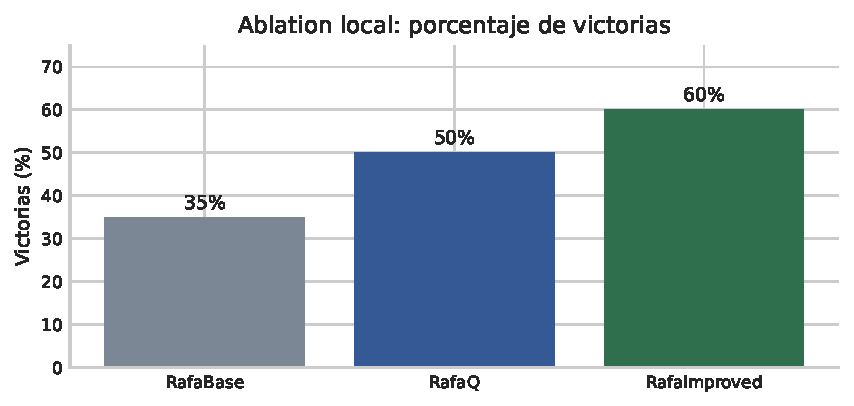
\includegraphics[width=0.56\linewidth]{figures/winrate_versions.pdf}\\[-4pt]
\small \textbf{Figura 1.} Porcentaje de victorias en comparación local entre versiones.
\end{center}

\section*{Validación mínima}
El desempeño se midió en función del oponente, no como un único número global. Contra el jugador aleatorio, las tres versiones ganaron el \textbf{100\%} de 20 partidas como rojo y 20 como amarillo, sin derrotas. Esto cumple el prerrequisito del reto. También se evaluó el autodesempeño: cada versión jugando contra una copia exacta de sí misma. En RafaImproved aparecen más empates (20\%), lo cual indica una política más estable cuando ambos lados aplican la misma estrategia.

\begin{center}
\begin{minipage}{0.48\linewidth}
\centering
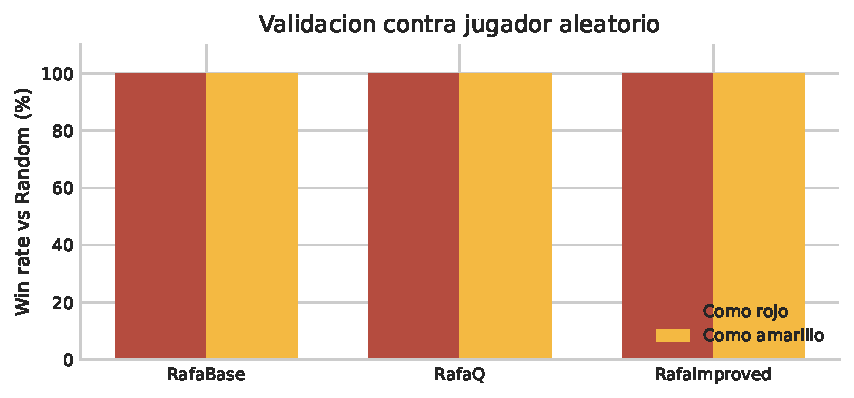
\includegraphics[width=\linewidth]{figures/random_versions.pdf}\\[-4pt]
\small Random por versión y color.
\end{minipage}
\hfill
\begin{minipage}{0.48\linewidth}
\centering
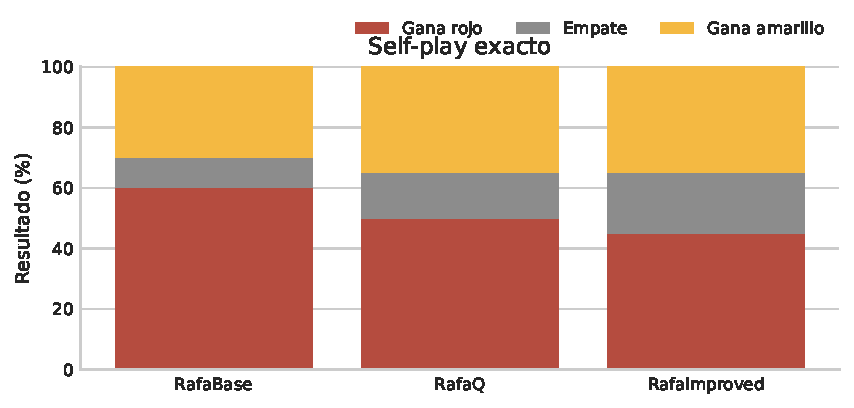
\includegraphics[width=\linewidth]{figures/selfplay_versions.pdf}\\[-4pt]
\small Self-play exacto.
\end{minipage}\\[-2pt]
\small \textbf{Figura 2.} Validación mínima: Random y self-play exacto.
\end{center}

\section*{Sweep y uso de memoria}
Para analizar configuración y recursos, se varió \texttt{total\_time} (presupuesto online por partida) y \texttt{global\_prior\_visits} (peso de la memoria en UCB). El mejor punto observado contra RafaQ fue \textbf{prior=10} y \textbf{2s}, con 100\% de victorias en esa muestra. La conclusión no es que más tiempo siempre gane, sino que el peso de la memoria debe calibrarse: muy bajo ignora experiencia y muy alto puede sobreconfiar en estimaciones ruidosas.

\begin{center}
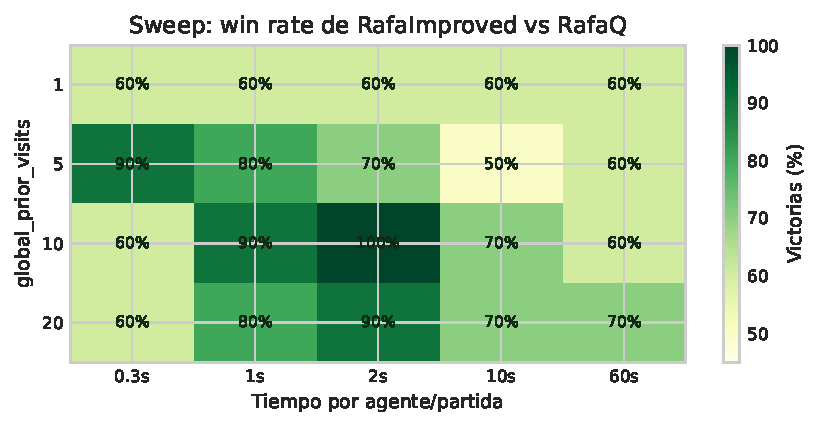
\includegraphics[width=0.56\linewidth]{figures/sweep_improved_vs_q_winrate.pdf}\\[-4pt]
\small \textbf{Figura 3.} Sweep de RafaImproved vs RafaQ en porcentaje de victorias.
\end{center}

La cobertura aproximada de estados vistos cae fuertemente a medida que avanza la partida. Esto muestra que, aunque la Q-table es grande, muchos estados de medio/final de partida siguen dependiendo de búsqueda online.

\begin{center}
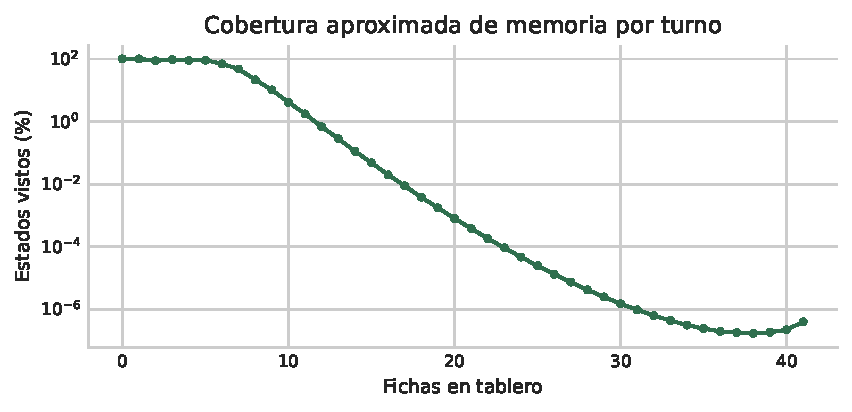
\includegraphics[width=0.56\linewidth]{figures/memory_coverage.pdf}\\[-4pt]
\small \textbf{Figura 4.} Porcentaje aproximado de estados vistos por número de fichas.
\end{center}

\section*{Conclusiones y mejoras}
RafaImproved supera a RafaQ porque no solo recuerda valores, sino que hace rollouts de mayor calidad y decide de forma más robusta. Sin embargo, el análisis muestra que el límite principal no es Random, sino la cobertura: en partidas avanzadas hay demasiados estados posibles y la memoria empieza a ser dispersa. Cuando eso ocurre, el agente vuelve a depender casi totalmente de la búsqueda online del turno.

La mejora más directa es \textbf{canonicalizar simetría horizontal}. En Connect-4, muchas posiciones son equivalentes a su espejo; hoy se guardan como estados distintos, duplicando aprendizaje. También conviene entrenar \textbf{posiciones de medio/final de partida}: en lugar de iniciar todos los self-play desde tablero vacío, se pueden muestrear estados intermedios y reforzar justo las profundidades donde la cobertura cae. Finalmente, se deberían guardar \textbf{trayectorias compactas} en evaluación para medir el hit-rate real: no solo cuántos estados existen en la Q-table, sino cuántas decisiones de torneo realmente encuentran memoria útil.

\end{document}
